Electrical Vehicles (EVs) have been scoped as the transition transportation technology to replace internal combustion engine vehicles (ICEVs) \cite{Kester2018PromotingDiffusion, Ajanovic2018ElectricProblem}, however, despite academic consensus, the deployment of EVs remains low with a representation of, less than 1\% of the combined global vehicle fleet \cite{InternationalEnergyAgencyIEA2017GlobalCounting}. Multiple reasons for the slow transition have been examined ranging from battery performance \cite{Ajanovic2018ElectricProblem}, vehicle costs \cite{Sovacool2017TheAgenda}, range limitations \cite{Noel2019FearAnxiety}, etc., and are frightening similar as determined a decade ago \cite{Sovacool2009BeyondTransition}. Simultaneously, advocates for EVs have been using the arguments of vehicle-to-grid (V2G), which enables strategic storing and exchange of electricity \cite{Sovacool2017TheAgenda}. However, few, if any studies have adequately examined the potential usage of EVs and EV batteries after the expired lifetime in combination with multi-megawatt wind turbines. Instead recent studies have focused on the combination of PV and retired EV batteries, and found that a) residual capacities can be exploited \cite{HUANG201980}, b) power management and selection strategies are required to optimize the value of the retired battery \cite{8279474}, and c) the environmental, social and economic profiles of EV batteries are improved due to a minimization of the recycling rate \cite{TANG20194304}. Assuming the same consequences for retired EV batteries, it 
would inevitably increase the value of lifetime EVs, and potentially add to the policy mechanisms, which especially seems to be lacking in Denmark \cite{Kester2018PromotingDiffusion}. As a matter of fact, only  8,746 EVs (plug-in hybrids and all-electric vehicles) were registered in Denmark by the end of 2017 \cite{Bilimp}, which is far less than the Scandinavian neighbours Norway (209,122)  \cite{Elbil} and Sweden (50,304) \cite{BilSweden}. This being despite the fact that Denmark has excellent wind resources \cite{Enevoldsen2016OnshoreRisks},  a high penetration of wind power in its electricity mix (44\% of the demand in 2017) \cite{Pineda2018}, and several days with a surplus of electricity and thereby negative electricity prices \cite{Hou2017OptimizingDenmark}.

Using batteries for electrical storage system (ESS) is not a novel thought, and especially lithium-ion battery was brought up in several studies as a prominent technology for load shifting and peak shaving demands \cite{Luo2015OverviewOperation, Zakeri2015Corrigendum569596,Wen2018Multi-time-scaleStorage, Fang2018DynamicSystems}, and highlighted for its capabilities of low standby losses and high energy efficiencies (60 - 95\%) \cite{Chen2009ProgressReview}. Using batteries to increases the profitability of wind farms have also been proposed before \cite{Hou2018CooperationMarkets}, as several studies demonstrated methods for lucrative bidding strategies on the day-ahead markets when combining batteries and wind farms \cite{Baringo2016OfferingApproach, Dai2015OptimalMarket}. Furthermore, applying batteries as the cornerstone technology in ESS was concluded to be the most profitable approach to provide primary frequency service in the Danish reserve electricity market almost a decade ago \cite{Jozef2011AalborgA}.

This study will investigate solutions to a) The fluctuations in Danish electricity prices due to the heavy reliance on wind power, and b) The investment opportunities of installing retired EV batteries in Danish operational offshore wind farms. 

\begin{figure*}
\centering
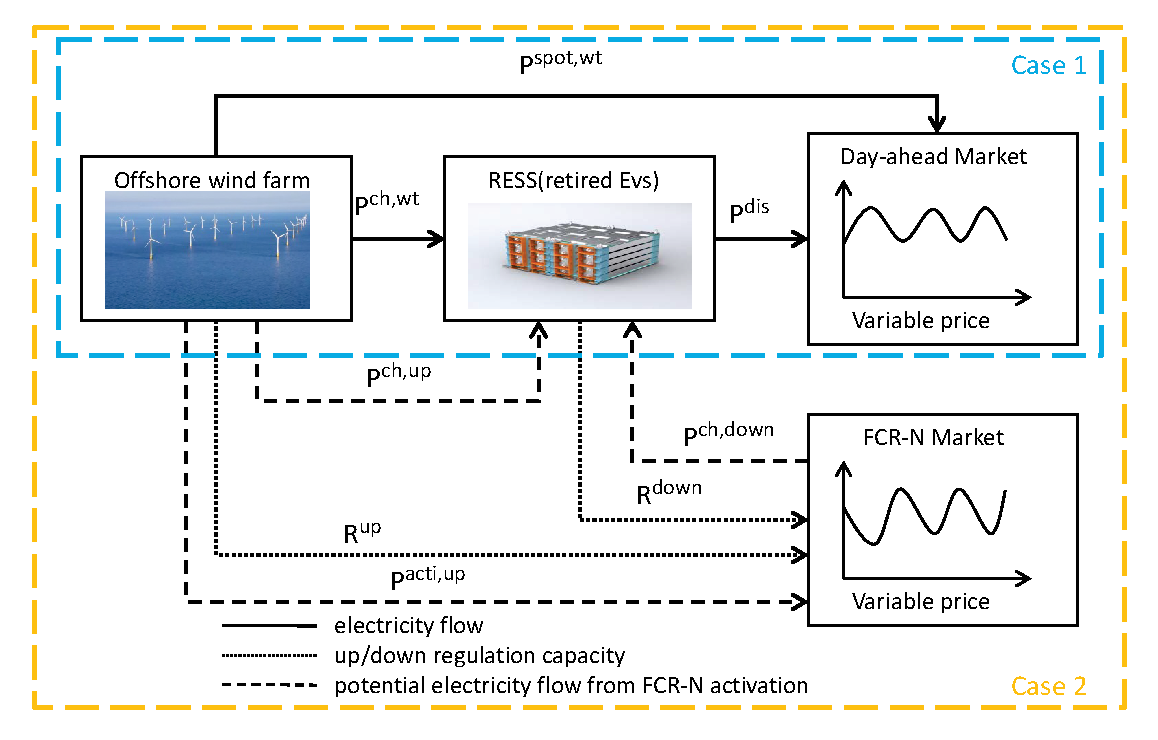
\includegraphics[width = 0.8\textwidth]{figures/model.eps}
\caption{Hybrid wind farm-RESS system schematic layout}
\label{fig:model}
\end{figure*}

In order to examine such challenges, the hybrid wind farm - retired EV batteries system is expected to participate in both the day-ahead and the FCR-N market. As a comparison, another case in which the wind farm only participates in the spot market is also studied, both shown in Fig. \ref{fig:model}. According to the rule of Danish transmission system operating, the balance responsible parties (BRPs, referring to the hybrid system in this study) merely need to provide a small amount of energy to mitigate the frequency deviation and get remunerated mainly by the bidden power capacity. Therefore, the electricity generated from the wind turbines can be sold at the spot market or caters for upward regulations of the FCR-N market, with part energy or the surplus going into the RESS or possibly both.

Since discharging the battery will incur high cost and reduce the battery lifetime and performance
obviously, the RESS works as downward regulation medium and receives electricity from the FCR-N market when downward regulation is needed. The upward regulation in the FCR-N market can be handled by controlling the wind turbines in the de-rated mode and releasing those when needed. 

The research materials and methods are based upon the examination of the potential profitability of integrating retired EV batteries in a Danish operational offshore wind farm. Furthermore, web searches have been conducted to inform about statistics of EVs and the market prices in Denmark. The following sections describes the methodology and materials applied for the core elements of this research. 